\subsection{Switch drivers}

\begin{frame}{Ethernet switches in Linux}
	\begin{itemize}
		\item The \textbf{switchdev} framework allows configuring the \textbf{switching fabric}
		\item Switch ports are represented as regular \code{net_device}
	\end{itemize}
	\begin{center}
		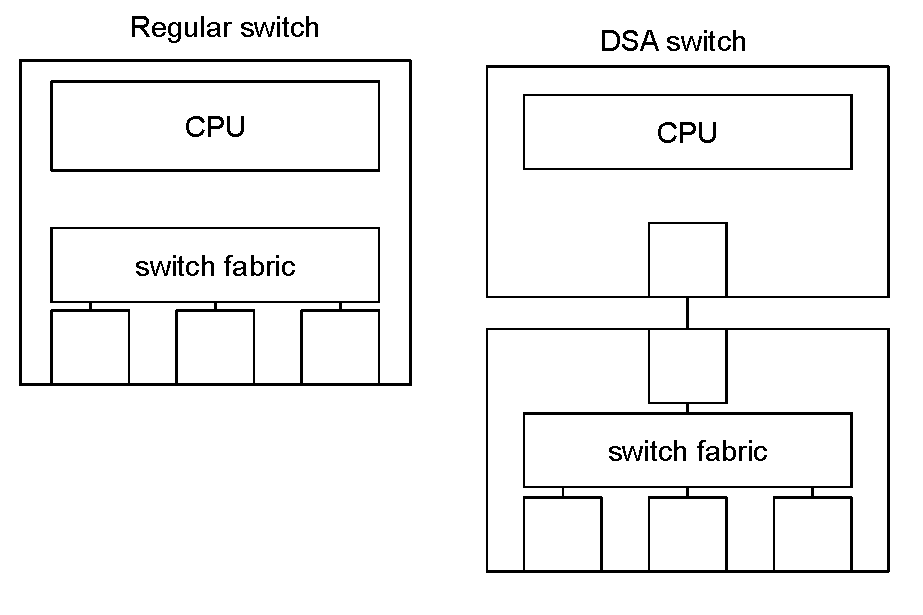
\includegraphics[width=0.6\textwidth]{slides/networking-driver-switch/switches.pdf}
	\end{center}
\end{frame}

\begin{frame}{Ethernet switches in Linux}
	\begin{itemize}
		\item By default, without any further configuration, each port is \textbf{independent}
		\item As each port has their \code{net_device}, they have their own \code{net_device_ops}
		\item Non-DSA switches are just regular Ethernet drivers, with extra logic for switchdev
		\item DSA switches have their ports handled by the \href{https://elixir.bootlin.com/linux/v6.15.2/source/net/dsa/port.c}{DSA port} infrastructure
			\begin{itemize}
				\item Implements the \code{.ndo_start_xmit}
			\end{itemize}
	\end{itemize}
\end{frame}

\begin{frame}{Switchdev}
	\begin{columns}
	 \column{0.4\textwidth}
		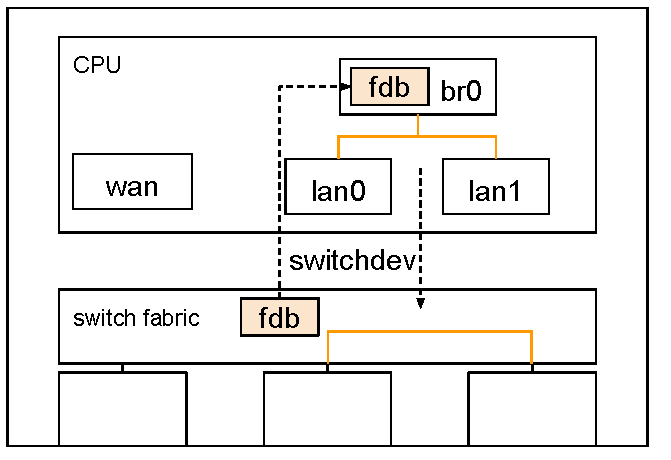
\includegraphics[width=\textwidth]{slides/networking-driver-switch/switchdev.pdf}
	 \column{0.6\textwidth}
	\begin{itemize}
		\item \textbf{switchdev} is a framework allowing drivers to implement switching configuration ops
		\item Bridging, VLANs, filtering, queueing, redirection, snooping, etc.
		\item The hardware \textbf{must} be able to report internal reconfiguration events
	\end{itemize}
	\end{columns}
\end{frame}

\begin{frame}{Notifiers}
	\begin{itemize}
		\item Drivers don't implement any kind of \code{switchdev_ops}
			\begin{itemize}
				\item Switch-related events don't specifically target a single \code{netdev}
			\end{itemize}
		\item Drivers instead subscribe to \textbf{kernel notifications} through \code{notifiers}
		\item Userspace bridging configuration triggers reconfiguration events
			\begin{itemize}
				\item \ksym{NETDEV_CHANGEUPPER} : A \code{netdev} has a new \code{upper_dev}
				\item \ksym{BR_STATE_FORWARDING} : A \code{bridge port} is set in forwarding state
			\end{itemize}
		\item The switch reports internal events, that the driver notifies to the kernel
			\begin{itemize}
				\item \kfunc{call_switchdev_notifiers}
			\end{itemize}
	\end{itemize}
\end{frame}

\begin{frame}[fragile]{Switchdev notifiers - example}
	\begin{block}{switchdev example}
		{\fontsize{7}{8}
	\begin{minted}{c}
static int adin1110_switchdev_event(struct notifier_block *unused,
                                    unsigned long event, void *ptr)
{
    if (!adin1110_port_dev_check(netdev))
        return NOTIFY_DONE;

    switch (event) {
    case SWITCHDEV_FDB_ADD_TO_DEVICE:
    case SWITCHDEV_FDB_DEL_TO_DEVICE:
        /* Add item to FDB */
    }

    return NOTIFY_DONE;
}

static struct notifier_block adin1110_switchdev_notifier = {
    .notifier_call = adin1110_switchdev_event,
};

static int adin1110_setup_notifiers(void)
{
    register_switchdev_notifier(&adin1110_switchdev_notifier);
}
\end{minted}
	}
	\end{block}
\end{frame}

\begin{frame}{Switchdev notifications}
	\begin{itemize}
		\item \code{NETDEV_CHANGEUPPER} : A \code{netdev} was added to or removed from a bridge
		\item \code{SWITCHED_FDB_ADD_TO_DEVICE} : A FDB entry was added by user
		\item \code{SWITCHED_PORT_OBJ_ADD} : Generic notifier to add an entry to a port
			\begin{itemize}
				\item \code{SWITCHDEV_OBJ_ID_PORT_VLAN} : A port belongs to a VLAN
				\item \code{SWITCHDEV_OBJ_ID_PORT_MDB} : Add a Multicast address to a port
			\end{itemize}
		\item Drivers notify the kernel when the operation could be offloaded
			\begin{itemize}
				\item \textit{e.g.} \code{call_switchdev_notifiers(SWITCHDEV_FDB_OFFLOADED, ndev, &info.info, NULL);}
			\end{itemize}
	\end{itemize}
\end{frame}

\begin{frame}{DSA}
	\center{\textbf{D}istributed \textbf{S}witch \textbf{A}rchitecture}
	\begin{columns}
	\column{0.2\textwidth}
		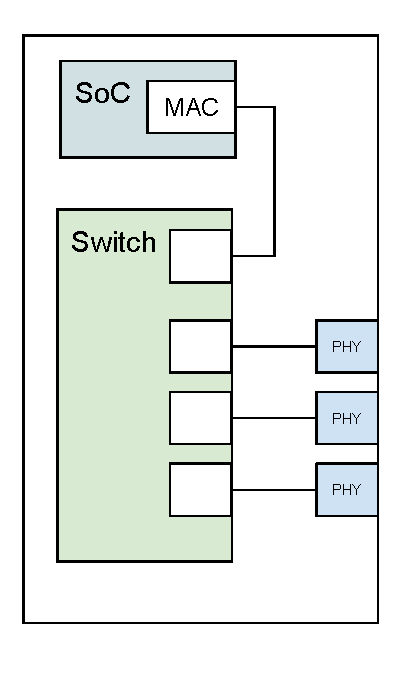
\includegraphics[width=\textwidth]{slides/networking-driver-switch/DSA.pdf}
	\column{0.8\textwidth}
	\begin{itemize}
		\item Mainly used by dedicated switch chips
		\item One or more ports are connected to SoC interfaces
		\item DSA switches may be chained together
		\item The CPU to Switch link is called the \textbf{cpu conduit} or \textbf{cpu port}
		\item Switch to Switch links are called \textbf{dsa conduits}
		\item Other interfaces are called \textbf{user} ports
		\item Frames on \textbf{conduits} are often \textbf{tagged} to identify the destination port
		\item DSA \textbf{uses} switchdev, and does not replace it
	\end{itemize}
	\end{columns}
	%schema
\end{frame}

\begin{frame}{DSA tagging}
	\begin{columns}
	\column{0.5\textwidth}
		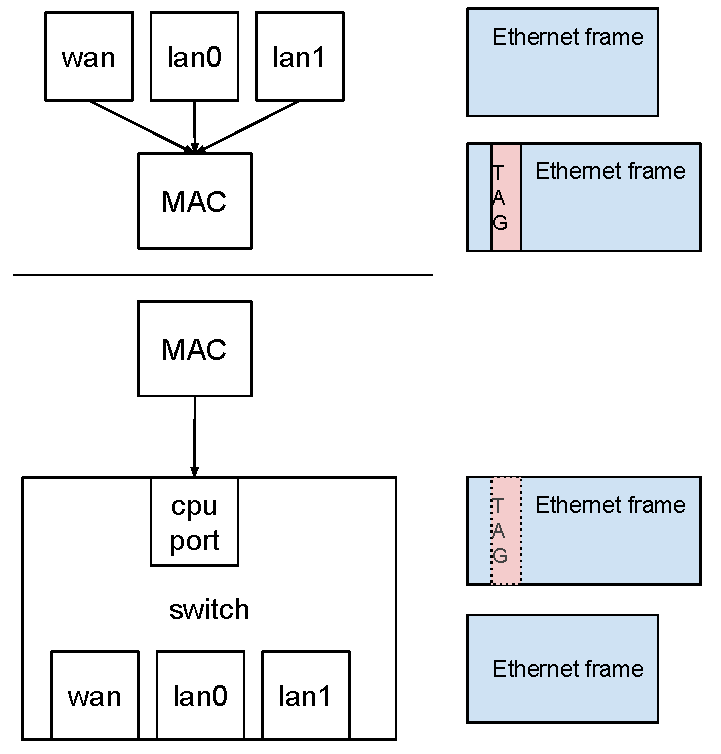
\includegraphics[width=\textwidth]{slides/networking-driver-switch/dsa_tagging.pdf}
	\column{0.5\textwidth}
	\begin{itemize}
		\item A vendor-specific TAG is added to the frame
		\item It contains the identifier of the egress port
		\item The frame is sent from the CPU to the switch
		\item The switch strips the tag and sends it to the port
		\item The opposite happens on receive
	\end{itemize}
	\end{columns}

\end{frame}

\begin{frame}[fragile]{DSA in devicetree}
	\begin{columns}
		\begin{column}{0.6\textwidth}
			\begin{block}{}
\begin{verbatim}
&mdio {
  switch0: ethernet-switch@1 {
    compatible = "marvell,mv88e6085";
    reg = <1>;
  
    dsa,member = <0 0>;
  
    ethernet-ports {
      #address-cells = <1>;
      #size-cells = <0>;
      [...]
    };
  };
};
\end{verbatim}
			\end{block}
		\end{column}
		\begin{column}{0.4\textwidth}
			\begin{itemize}
				\item \textbf{reg} : Address on the MDIO bus
				\item \textbf{dsa,member} : Position in the \textbf{cluster}, if applicable
				\item \textbf{ethernet-ports} : Contains the list of ports
			\end{itemize}
		\end{column}
	\end{columns}
\end{frame}

\begin{frame}[fragile]{DSA Ports in devicetree}
	\begin{columns}
		\begin{column}{0.5\textwidth}

\tiny
			\begin{block}{}
\begin{verbatim}
    ...
    ethernet-ports {
      switch0port0: ethernet-port@0 {
        reg = <0>;
        label = "cpu";
        ethernet = <&eth0>;
        phy-mode = "rgmii-id";
        fixed-link {
          speed = <1000>;
          full-duplex;
        };
      };
      
      switch0port1: ethernet-port@1 {
        reg = <1>;
        label = "wan";
        phy-handle = <&switch0phy0>;
      };

      switch0port2: ethernet-port@2 {
        reg = <2>;
	link = <&switch1port0>;
      };

      ...      
    };
    ...
\end{verbatim}
			\end{block}
		\end{column}
		\begin{column}{0.5\textwidth}
			\begin{itemize}
				\item \textbf{reg} : Port number
				\item \textbf{label} : Port name, will become the interface name
				\item \textbf{ethernet} : phandle to the CPU-side MAC interface
				\item \textbf{link} : phandle to another DSA switch's port, for cascading
				\item PHY mode and phandle
			\end{itemize}
		\end{column}
	\end{columns}
\end{frame}



\begin{frame}[fragile]{Tagging}
	\begin{itemize}
		\item Tagging happens outside of the switch driver, in a dedicated tagger : \code{net/dsa/tag_*.c}
		\item Some switches support multiple tagging formats
			\begin{itemize}
				\item It can be specified in \textbf{devicetree}
			\end{itemize}
	\end{itemize}
	\begin{block}{DSA tagger}
		\begin{minted}{c}
static const struct dsa_device_ops foo_ops = {
    .name = "foo",
    .proto = DSA_TAG_PROTO_FOO,
    .xmit = foo_tag_xmit,
    .rcv = foo_tag_rcv,
    .needed_headroom = FOO_HDR_LEN,
    .promisc_on_conduit = true,
};
		\end{minted}
	\end{block}
\end{frame}

\begin{frame}{Chaining}
	\begin{itemize}
		\item Some DSA switches can be daisy-chained
		\item The ports that link switches together have no associated \code{net_device}
	\end{itemize}
	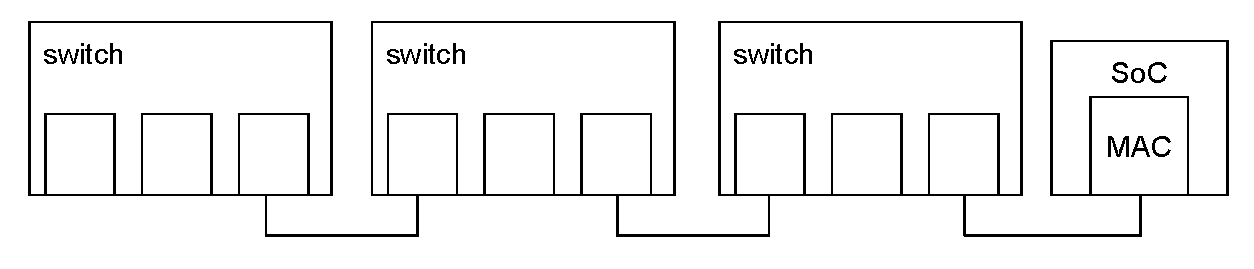
\includegraphics[width=\textwidth]{slides/networking-driver-switch/chained.pdf}
\end{frame}

% Switchdev and ops
% DSA and tagging
